\chapter{Benutzeranleitung}

\hypertarget{missionlist}{\section{Missionsliste}}

\begin{figure}[H]
	\centering
	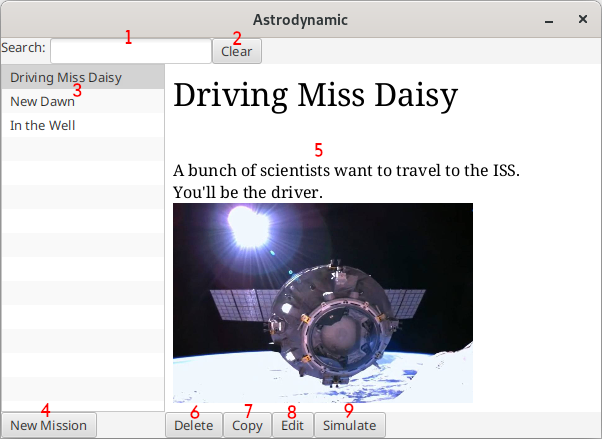
\includegraphics[width=12cm]{res/missionsliste.png}
	\caption{GUI Missionsliste mit Annotation}
\end{figure}

\begin{enumerate}[noitemsep]
	\item Suchfeld
	\item Clear: Suchfeld leeren
	\item Liste verfügbarer Missionen
	\item New Mission: Neue Mission öffnen im Missions-Editor
	\item Beschreibung der ausgewählten Mission
	\item Delete: Ausgewählte Mission löschen
	\item Copy: Ausgewählte Mission kopieren
	\item Edit: Ausgewählte Mission öffnen im Missions-Editor
	\item Simulate: Ausgewählte Mission öffnen im Simulator
\end{enumerate}

\subsection{Grundlagen}
Die Missionsliste ist der Einstiegsbildschirm beim Start des Programs.
Hat der Benutzer keine Mission gespeichert welche geladen werden kann so werden drei Testmissionen geladen.
Am linken Rand befindet sich die Liste der verfügbaren Missionen.Anwählen einer Mission in der Liste per Klick mit der Linken Maustaste lädt die Missionsbeschreibung in den rechten Anzeigebereich und ermöglicht mit diese Mission per Buttons unten rechts am Bildschirmrand weiter zu Interagieren.

\subsection{Missionen nach Beschreibung suchen}
Das Suchfeld führt eine sofortige Textsuche auf Missions-Name und -Beschreibung durch und zeigt auf Basis dieser nur passende Missionen in der Liste der verfügbaren Missionen. Durch drücken des Clear-Buttons können längere Sucheingaben sofort gelöscht und die Sortierung zurückgesetzt werden.

\begin{figure}[h]
	\centering
	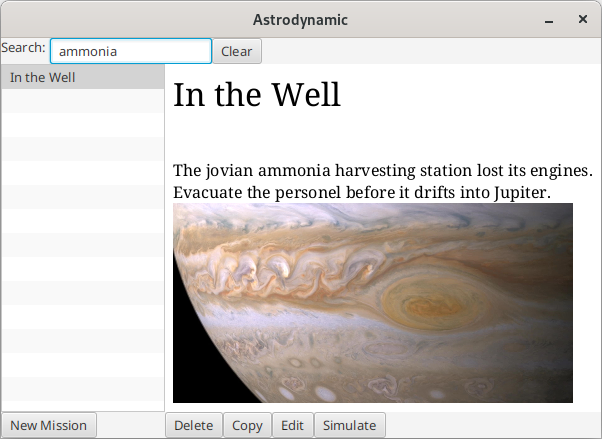
\includegraphics[width=8cm]{res/search.png}
	\caption{Missionsfilter bei Suche nach 'ammonia'}
\end{figure}

\subsection{Anlegen einer neuen Mission}
Klicken sie auf den ''Neue Mission öffnen im Missions-Editor''-Button unten links.
Es öffnet sich nun der Missions-Editor.
Für Details zum editieren einer Mission konsultieren sie das \hyperlink{missioneditor}{Kapitel Missions-Editor}.

\subsection{Löschen einer Mission}
Wählen sie die Mission aus der Liste der verfügbaren Missionen per Mausklick aus.
Klicken sie auf Delete.
Ein Popup öffnet sich mit der Löschanfrage.

\begin{figure}[H]
	\centering
	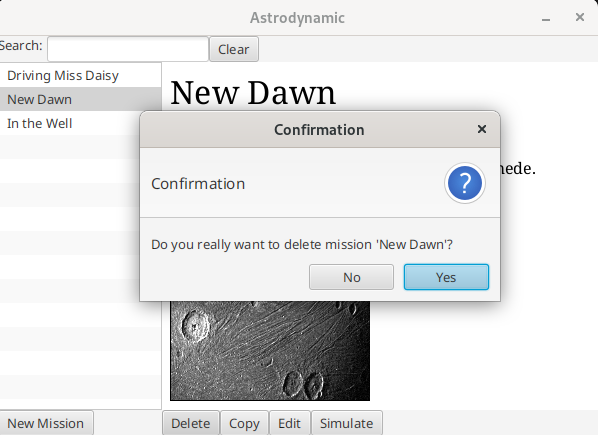
\includegraphics[width=8cm]{res/loeschen.png}
	\caption{Sicherheitsabfrage bei Missionslöschung}
\end{figure}

Bestätigen sie das Popup mit Klick auf Yes.
Die Mission wird aus der Liste der verfügbaren Missionen entfernt.

\subsection{Kopieren einer Mission}
Wählen sie die Mission aus der Liste der verfügbaren Missionen per Mausklick aus.
Klicken sie auf Copy.
Es öffnet sich nun der Missions-Editor mit der kopierten Mission.
Für Details zum editieren einer Mission konsultieren sie das \hyperlink{missioneditor}{Kapitel Missions-Editor}.

\subsection{Editieren einer Mission}
Wählen sie die Mission aus der Liste der verfügbaren Missionen per Mausklick aus.
Klicken sie auf Edit.
Es öffnet sich nun der Missions-Editor mit der ausgewählten Mission.
Für Details zum editieren einer Mission konsultieren sie das \hyperlink{missioneditor}{Kapitel Missions-Editor}.

\subsection{Simulieren einer Mission}
Wählen sie die Mission aus der Liste der verfügbaren Missionen per Mausklick aus.
Klicken sie auf Simulate.
Es öffnet sich nun der Simulator mit der ausgewählten Mission.
Für Details zum simulieren einer Mission konsultieren sie das \hyperlink{simulator}{Kapitel Simulator}.